\section{Introduction}
\label{sec:introduction}

\begin{figure}[t]
\centering
\includegraphics[width=0.5\textwidth]{ECGExp.eps}
\caption{ Five ECG time-series corresponding to three different diseases. Different color denotes different diseases.}
\label{fig:ecgexample}
\end{figure}

\begin{figure}[t]
\centering
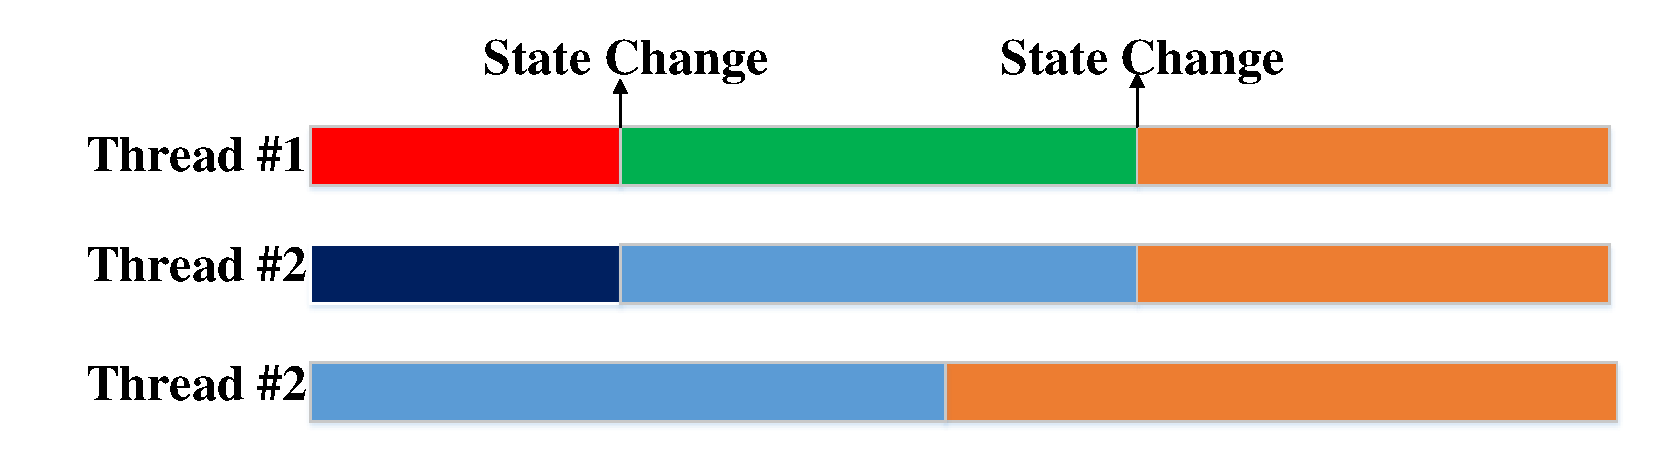
\includegraphics[width=0.50\textwidth]{HPCExample.pdf}
\caption{Snapshot of HPCToolket Traceviewer of an environment simulation task.
Each line represent one thread, \textbf{Thread0} to \textbf{Thread3} belongs to a Ocean Simulation Program, and \textbf{Thread4} to \textbf{Thread8} belongs to a Weather Simulation Program. Different Color in each thread denotes the ``Call Path" state.}
\label{fig:hpcexample}
\end{figure}

The focus of this paper will be on the time series data. A time series is defined as a sequence of values $\{s_1,s_2,...,s_m\}$
associated with timestamps $\{t(s_1), t(s_2),..., t(s_m)\}$, which has the relationship of $t(s_i) = t(s_{i-1})+\tau$, where $\tau$is the sampling interval, and $m$ is the number of points in the time series.

Time series mining is ubiquitous in data driven applications including robotics, medicine~\cite{oates2000method,caracca2000discovering}, speech~\cite{rabiner1993fundamentals}, object detection in vision~\cite{yang2002detecting, sonka2014image}, system failure diagnosis~\cite{luo2014correlating,sun2014querying}, Earth Science \cite{mudelsee2013climate}, Finance \cite{granger2014forecasting}, etc.

Due to its pervasive presence, time series mining have received significant attention in recent years. A common prerequisite for data mining algorithms, such as clustering, search, classification and regression, etc., is a measure of correlation (or similarity). Dynamic Time Warping (DTW) is widely accepted, and arguably the most popular, measure of similarity (or correlation) for time series data in general~\cite{rakthanmanon2012searching, muller2007dynamic, chen2013dtw}.

All existing measures over time series, including the popular DTW, relies on the notion that two time series $S_1$ and $S_2$ are similar, if there is a long enough similarly behaving subsequence common between them. This is a very reasonable notion which is also the desired nature of the similarity function in many applications.  However, there are plenty of real-world problems where the notions of similarity can be very different. Using existing similarity measures, such as DTW or Euclidean distance, for such problems often lead to misleading results. Despite their importance, there has been little previous work addressing those scenarios. To signify their importance, we provide two motivating real-world examples:


\textbf{Analysis of ECG (Electrocardiogram) data}

Electrocardiography \cite{holter1961new} (ECG or EKG*)
is the process of recording the electrical activity of the heart over a period of time using electrodes placed on a patient's body.
These electrodes detect the tiny electrical changes on the skin that arise from the heart muscle depolarizing during each heartbeat.
The tiny electrical changes occurs in different rhythm corresponds to different heart physical states or different diseases. 
If two ECG often have tiny electrical changes at the same time, they can be represent correlation between the corresponding body (e.g. same disease or same heart physical state, etc).\cite{marriott1988practical}.

%, 

Fig. \ref{fig:ecgexample} shows five ECG time series, and these five ECG comes from three diseases.
By using DTW distance, DTW distance between ECG1 and ECG2 is $0.2$, while the distance between ECG2 and ECG3 is $0.5$.
It is not surprising that using DTW for such problems lead to misleading results.
This because that the similarity of ECG time series data correspond to the change rhythm, not correspond to the point to point similarity.
Since the ECG time series data have different change patterns (e.g. Increase-Decrease, Decrease-Increase, or a Sudden wave, etc.). These different change patterns can effect the performance of point to point similarity measures.

On the other hand, By using the similarity in this work, the correlation between ECG1 and ECG2 is $1.00$, and the similarity between ECG1 and ECG3 is $0.25$, which is the result exactly what we need.

%

%We choose three time series from two different labels in that data set.
%We illustrate this in Figure\ref{fig:ecgexample}, where we show the hierarchical clustering of these three time series under various measures. 
%Top two red bold time series ($ECG\#1,ECG\#2$) are labeled as same class, and $ECG \#3$ is labeled as other class.




%correlation is a major research topic in data mining area.
%Such correlating techniques has been applied in many real world problems.
%For example, some researchers use time series correlation techniques to analysis the signal information for speech processing \cite{rabiner1993fundamentals}.
%Image processing researchers also use time series correlation techniques to deal with the image retrieval problems and object detection problems \cite{yang2002detecting, sonka2014image}.
%In the system diagnose area\cite{luo2014correlating,sun2014querying}, time series correlation techniques also widely used to mine the system behavior and diagnose system failures.
%Time series correlation techniques can also be used for analyzing bio-sequences (e.g DNA Sequence, etc \cite{mount2001bioinformatics} etc.

%In addition, real world time series are all high dimensional and large scale data, how to mining such huge amount of data set is also a challenge for us.
%By analyzing such data, one can find some useful information hidden behind the human body, thus to uncover some miracles of human body \cite{tilley1979essentials}.
%The first real-world example is ECG data\cite{holter1961new}. 


\textbf{Analysis of HPC Thread time series.}
High-performance computers (HPC) have become enormously complex. Today, the largest systems consist of more than tens of thousands of nodes. Nodes themselves are equipped with one or more multicore microprocessors\cite{adhianto2010hpctoolkit}. 
High-performance computer can generate over billions of threads during running.
And how to automatically analysis and monitoring the HPC is a major task for HPC researchers \cite{mccurdy2010memphis,tallent2009effective}.

%As a result, it is increasingly difficult for application developers writing complex scientific programs to attain a significant fraction of peak performance on modern microprocessor-based computer systems.

HPCToolkit\footnote{http://hpctoolkit.org/} can be used to generate the performance information of each thread from High performance computers. 
And each thread can be represented as a time series. The value of the time series denote the call path \cite{adhianto2010hpctoolkit} state of the thread.

%(Depend on which aspect of a thread to be represent, domain knowledge required) The thread change information (e.g. change from one state to another state) can directly reflect some important properties of different threads.

Fig. \ref{fig:hpcexample} shows a example of five thread time series data. Different colors means different call path state. 
\textbf{Thread0} to \textbf{Thread3} belongs to a Ocean Simulation Program, and \textbf{Thread4} to \textbf{Thread8} belongs to a Weather Simulation Program. Different Color in each thread denotes the ``Call Path" state.

It is obvious that threads from the same program are highly correlated. This correlation can be detected by the existing method such as Pearson correlation or DTW distance. For example, the DTW distance between Thread 0 and Thread 1 is $0.05$, which denotes they are highly correlated.

However, for the Environment Simulation Task, Ocean simulation Program and Weather Simulation Program are also correlated with each other. Because in the real world, the weather earth are correlated with the activities of the ocean.  So these two programs often change data during simulating, when they change data, they will change state at the same time.

And this type of correlation (Threads Correlation between Different Programs) can not be detected using DTW distance. For example, the DTW distance between Thread 0 and Thread 4 is $0.8$. While using our method, we can find a $0.6$ correlation coefficient with each other.

We can see that DTW and Euclidean distance can not perform well. Because threads in the different program always have different states and DTW and Euclidean will regard these state difference as large distance.
On the other hand, change based correlation only consider the change information of the time series, and the state difference between different threads of each program can not bias the correlation result.


%However, in most real world problems, time series data often have different patterns (Heterogeneous time series). For example, in the area of system analysis area.
%Each performance counter can be regarded as a time series (e.g. CPU Usage, Memory Usage, etc.).
%Some of the time series may be a periodical time series, but others may be a linear or random patterns.
%However, heterogeneous time series may also be correlations between each other.
%So, how to calculate the correlation between heterogeneous time series data is a challenge.

As showed in above examples, the existing point to point time series similarity measures (e.g. L1-Distance, L2-Distance \cite{han2011data}, and DTW-Distance \cite{muller2007dynamic}, etc) or correlation measures (e.g. Pearson Correlation \cite{pearson1904mathematical}, Kendall rank correlation \cite{kendall1938new}, and Spearman's rank correlation \cite{pirie1988spearman}, etc.) can not deal with time series similarity problem when time series have heterogeneous patterns. 
The reason is: for heterogeneous time series, the correlation information is often associated with the change (During a period of time) of time series, rather than a point-to-point relationship in the traditional correlation analysis techniques. We will introduce the related research of point to point based similarity measure in detail in Section \ref{sec:relatedwork}.

As a result, in order to deal with heterogeneity properties of time series, we proposed a change based correlation coefficient. 
Our change based correlation method firstly extract the change information of the time series data, and then use the change information to calculate the correlation coefficient between the two time series.
By taking the advantage of this correlation coefficient, we propose to use LSH method to dealing with very large top-k searching problems.

The contribution of this paper is listed as follow:
\begin{enumerate}
\item Motivated by real applications, we investigate the correlation
problem as between heterogeneous time series .
To the best of our knowledge, this is the first attempt
to evaluate the correlation between time series with different patterns.

\item We proposed a correlation coefficient between heterogeneous time series. By taking the advantage of this correlation coefficient, we can do searching and mining on large scale time series datasets.


\item The experiments on Synthetic data sets and Real world data sets show the effectiveness and efficiency of our method.
\end{enumerate}

The rest of the paper is organized as follows: In Section 2, we introduce the problem
statement and formulation. Our approach is proposed in Section 3. The Empirical evaluation is shown in Section 4. In Section 5, we introduce some
related works. Finally, we conclude our work in Section 6.



